\subsection{Simulation-based Evaluation}

\begin{table*}[htbp]
    \centering
    \begin{tabular}{ccccccc}
        \toprule

        \multicolumn{7}{c}{\textbf{Mean Absolute Error (MAE)}}                                                                      \\
        \midrule

        \textbf{Scenario} & \textbf{Var.} & PA     & GLM                & MLP-3/2         & MLP-16/8           & MLP-32/16          \\
        \midrule

        Epi-1             & \( R_t \)     & 0.11   & \underline{0.052}  & \textbf{0.032}  & 0.058              & 0.065              \\[6pt]

        Epi-2             & \( R_t \)     & 0.048  & \textbf{0.0064}    & 0.038           & \underline{0.0075} & 0.017              \\[6pt]

        Epi-3             & \( R_t \)     & 0.055  & 0.12               & 0.084           & \underline{0.054}  & \textbf{0.036}     \\[6pt]

        Epi-4             & \( M \)       & 0.011  & 0.0085             & 0.0068          & \textbf{0.0031}    & \underline{0.0045} \\[6pt]

        \multirow{3}{*}{FBD-1}
                          & \( \lambda \) & 0.12   & 0.032              & \textbf{0.018}  & 0.025              & \underline{0.023}  \\
                          & \( \mu \)     & 0.077  & \underline{0.0051} & \textbf{0.0039} & 0.017              & 0.027              \\
                          & Avg.          & 0.098  & \underline{0.019}  & \textbf{0.011}  & 0.021              & 0.025              \\[6pt]

        \multirow{3}{*}{FBD-2}
                          & \( \lambda \) & 0.075  & 0.030              & 0.026           & \underline{0.021}  & \textbf{0.020}     \\
                          & \( \mu \)     & 0.057  & 0.0088             & 0.022           & \textbf{0.0031}    & \underline{0.0072} \\
                          & Avg.          & 0.066  & 0.020              & 0.024           & \textbf{0.012}     & \underline{0.013}  \\[6pt]

        \multirow{3}{*}{FBD-3}
                          & \( \lambda \) & 0.061  & 0.16               & \textbf{0.011}  & \underline{0.015}  & 0.025              \\
                          & \( \mu \)     & 0.097  & 0.053              & \textbf{0.020}  & 0.025              & \underline{0.024}  \\
                          & Avg.          & 0.079  & 0.11               & \textbf{0.015}  & \underline{0.020}  & 0.025              \\[6pt]

        \multirow{3}{*}{FBD-4}
                          & \( \lambda \) & 0.13   & 0.025              & 0.021           & \underline{0.013}  & \textbf{0.011}     \\
                          & \( \mu \)     & 0.1754 & 0.0160             & 0.0261          & \underline{0.012}  & \textbf{0.0070}    \\
                          & Avg.          & 0.153  & 0.021              & 0.023           & \underline{0.013}  & \textbf{0.0090}    \\

        \bottomrule
    \end{tabular}
    \caption{Mean absolute error (MAE) across all scenarios for all inference frameworks considered (PA is the predictor-agnostic model). Bold indicates the best, underlined indicates the second-best.}%
    \label{tab:mae}
\end{table*}

\begin{table*}[htbp]
    \centering
    \begin{tabular}{ccccccc}
        \toprule

        \multicolumn{7}{c}{\textbf{Coverage}}                                            \\
        \midrule

        \textbf{Scenario} & \textbf{Var.} & PA   & GLM  & MLP-3/2 & MLP-16/8 & MLP-32/16 \\
        \midrule

        Epi-1             & \( R_t \)     & 0.93 & 0.96 & 0.98    & 0.99     & 0.98      \\[6pt]

        Epi-2             & \( R_t \)     & 0.95 & 0.98 & 0.98    & 0.99     & 0.98      \\[6pt]

        Epi-3             & \( R_t \)     & 0.96 & 0.75 & 0.91    & 0.98     & 0.98      \\[6pt]

        Epi-4             & \( M \)       & 0.91 & 0.35 & 0.79    & 0.97     & 0.90      \\[6pt]

        \multirow{3}{*}{FBD-1}
                          & \( \lambda \) & 0.90 & 0.90 & 0.97    & 0.98     & 0.98      \\
                          & \( \mu \)     & 0.97 & 0.96 & 0.97    & 0.97     & 0.93      \\
                          & Avg.          & 0.94 & 0.93 & 0.97    & 0.97     & 0.95      \\[6pt]

        \multirow{3}{*}{FBD-2}
                          & \( \lambda \) & 0.93 & 0.87 & 0.95    & 0.96     & 0.97      \\
                          & \( \mu \)     & 0.96 & 0.96 & 0.95    & 0.98     & 0.98      \\
                          & Avg.          & 0.94 & 0.91 & 0.95    & 0.97     & 0.97      \\[6pt]

        \multirow{3}{*}{FBD-3}
                          & \( \lambda \) & 0.96 & 0.23 & 0.85    & 0.87     & 0.92      \\
                          & \( \mu \)     & 0.97 & 0.32 & 0.73    & 0.73     & 0.78      \\
                          & Avg.          & 0.96 & 0.28 & 0.79    & 0.80     & 0.85      \\[6pt]

        \multirow{3}{*}{FBD-4}
                          & \( \lambda \) & 0.95 & 0.91 & 0.96    & 0.98     & 0.98      \\
                          & \( \mu \)     & 0.89 & 0.90 & 0.92    & 0.98     & 0.97      \\
                          & Avg.          & 0.92 & 0.91 & 0.94    & 0.98     & 0.97      \\

        \bottomrule
    \end{tabular}
    \caption{Coverage across all scenarios for all inference frameworks considered (PA denotes the predictor-agnostic model).}%
    \label{tab:coverage}
\end{table*}

\begin{table*}[htbp]
    \centering
    \begin{tabular}{ccccccc}
        \toprule

        \multicolumn{7}{c}{\textbf{Average 95\% CI Width}}                                 \\
        \midrule

        \textbf{Scenario} & \textbf{Var.} & PA    & GLM   & MLP-3/2 & MLP-16/8 & MLP-32/16 \\
        \midrule

        Epi-1             & \( R_t \)     & 0.96  & 0.35  & 0.29    & 0.51     & 0.67      \\[6pt]

        Epi-2             & \( R_t \)     & 0.89  & 0.34  & 0.36    & 0.50     & 0.63      \\[6pt]

        Epi-3             & \( R_t \)     & 1.1   & 0.42  & 0.44    & 0.62     & 0.76      \\[6pt]

        Epi-4             & \( M \)       & 0.041 & 0.014 & 0.021   & 0.022    & 0.020     \\[6pt]

        \multirow{3}{*}{FBD-1}
                          & \( \lambda \) & 0.44  & 0.14  & 0.11    & 0.17     & 0.22      \\
                          & \( \mu \)     & 0.45  & 0.11  & 0.093   & 0.13     & 0.15      \\
                          & Avg.          & 0.44  & 0.12  & 0.10    & 0.15     & 0.18      \\[6pt]

        \multirow{3}{*}{FBD-2}
                          & \( \lambda \) & 0.35  & 0.13  & 0.14    & 0.18     & 0.21      \\
                          & \( \mu \)     & 0.39  & 0.10  & 0.10    & 0.14     & 0.17      \\
                          & Avg.          & 0.37  & 0.12  & 0.12    & 0.16     & 0.19      \\[6pt]

        \multirow{3}{*}{FBD-3}
                          & \( \lambda \) & 0.40  & 0.17  & 0.16    & 0.20     & 0.22      \\
                          & \( \mu \)     & 0.39  & 0.071 & 0.074   & 0.088    & 0.095     \\
                          & Avg.          & 0.40  & 0.12  & 0.12    & 0.14     & 0.16      \\[6pt]

        \multirow{3}{*}{FBD-4}
                          & \( \lambda \) & 0.68  & 0.17  & 0.20    & 0.25     & 0.30      \\
                          & \( \mu \)     & 0.79  & 0.14  & 0.1775  & 0.24     & 0.28      \\
                          & Avg.          & 0.73  & 0.16  & 0.19    & 0.24     & 0.29      \\

        \bottomrule
    \end{tabular}
    \caption{Average 95\% credible interval width across all scenarios for all inference frameworks considered (PA denotes the predictor-agnostic model).}%
    \label{tab:avg_ci_width}
\end{table*}

\begin{table}[htbp]
    \centering
    \begin{tabular}{cccccc}
        \toprule
        \textbf{Scenario} & \textbf{PA} & \textbf{GLM} & \textbf{MLP-3/2} & \textbf{MLP-16/8} & \textbf{MLP-32/16} \\
        \midrule
        Epi-1             & 39878.25    & 30543.81     & 12750.74         & 6630.82           & 4586.71            \\
        Epi-2             & 58356.51    & 49470.21     & 13622.51         & 11485.42          & 8598.30            \\
        Epi-3             & 54439.66    & 43323.65     & 10997.51         & 11408.65          & 7643.71            \\
        Epi-4             & 162.19      & 175.93       & 137.84           & 106.11            & 79.70              \\
        FBD-1             & 57313.24    & 41452.32     & 12060.29         & 11601.46          & 7513.56            \\
        FBD-2             & 36272.02    & 23972.37     & 5120.69          & 5309.66           & 3614.67            \\
        FBD-3             & 29514.58    & 20281.02     & 1919.92          & 1770.44           & 1835.22            \\
        FBD-4             & 71.49       & 61.05        & 8.96             & 10.92             & 11.32              \\
        \bottomrule
    \end{tabular}
    \caption{Mean effective sample size (ESS) per hour across all scenarios and inference frameworks considered (PA denotes the predictor-agnostic model), averaged over all inference targets and all replicate trees for each scenario.}%
    \label{tab:mean_ess_per_hour}
\end{table}


\begin{figure}[htbp]
    \centering
    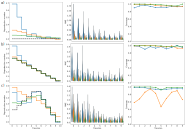
\includegraphics[width=1\textwidth]{figures/epi-skyline.pdf}
    \caption{Results for the epidemiological skyline scenarios: (a) Epi-1; (b) Epi-2; (c) Epi-3. For each inference framework—predictor-agnostic model (blue), GLM (orange), and the best-performing MLP in terms of MAE (Epi-1: MLP-3/2; Epi-2: MLP-16/8; Epi-3: MLP-32/16, shown in green)—the panels display, from left to right: the median reproduction number estimates across all replicate trees; the distribution of the mean absolute error (MAE) across trees; and the coverage of the 95\% credible intervals.}%
    \label{fig:epi-skyline}
\end{figure}

\begin{figure}[htbp]
    \centering
    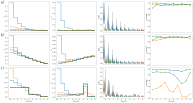
\includegraphics[width=1\textwidth]{figures/fbd-no-traits.pdf}
    \caption{Results for the birth–death skyline scenarios: (a) FBD-1; (b) FBD-2; (c) FBD-3. For each inference framework—predictor-agnostic model (blue), GLM (orange), and the best-performing MLP in terms of MAE (FBD-1: MLP-3/2; FBD-2: MLP-16/8; FBD-3: MLP-3/2, shown in green)—the panels show, from left to right: the median speciation rate (\( \lambda \)) estimates across all replicate trees; the median extinction rate (\( \mu \)) estimates across all replicate trees; the distribution of the mean absolute error (MAE) across trees for both rates combined; and the mean coverage of the 95\% credible intervals for the aggregated rates.}%
    \label{fig:fbd-skyline}
\end{figure}

Our implementation consistently matched or exceeded the performance of state-of-the-art phylodynamic models across a diverse range of simulation scenarios, as measured by all considered evaluation metrics. Table~\ref{tab:mae}, Table~\ref{tab:coverage}, and Table~\ref{tab:avg_ci_width} summarize the overall performance of the different inference methods across all scenarios and inference targets, in terms of mean absolute error (MAE), coverage, and average credible interval width, respectively. The Bayesian MLP approach reliably produced accurate parameter estimates with well-calibrated uncertainty, while remaining computationally feasible despite the additional inference cost.

In scenario Epi-1 (Figure~\ref{fig:epi-skyline}a), the inference target is a constant skyline reproduction number \( R_t \). The smallest MLP model tested MLP-3/2 (two hidden layers with 3 and 2 neurons), achieved the best performance, with a MAE of 0.032 and a high coverage of 0.98. It also demonstrated the highest precision, reporting the smallest average credible interval width of 0.29. The GLM model followed, with slightly lower performance (MAE:\ 0.052, coverage: 0.96, average CI width: 0.35), while the larger MLP architectures—MLP-16/8 and MLP-32/16—performed comparably to the GLM, with MAEs of 0.058 and 0.065, coverages of 0.99 and 0.98, and average CI widths of 0.51 and 0.67, respectively. The predictor-agnostic model performed the worst, with a MAE of 0.11; although coverage remained acceptable (0.93), its average credible interval width was very large (0.96). A similar pattern emerged for scenario FBD-1 (Figure~\ref{fig:fbd-skyline}a), which shares the same constant dynamics as the inference target. Here, the smallest MLP again outperformed all other models, followed by the GLM and the larger MLP architectures, which achieved performances similar to the GLM.\ The predictor-agnostic model again showed poor accuracy, coupled with very wide credible intervals despite reasonable coverage.

Figure~\ref{fig:epi-skyline}b corresponds to scenario Epi-2, in which the reproduction number \( R_t \) decreases linearly over time. In this setting, the GLM achieved the best performance, with a MAE of 0.0064, coverage of 0.98, and an average credible interval width of 0.34. The MLP-16/8 closely followed, showing a MAE of 0.0075, coverage of 0.98, and average CI width of 0.36. The larger MLP architectures also performed well, with MLP-32/16 achieving a MAE of 0.017 and coverage of 0.98, though with a wider average CI of 0.63. The smallest MLP, MLP-3/2, showed a higher MAE of 0.038, coverage of 0.98, and a narrow average CI width of 0.36. The predictor-agnostic model again performed the worst, with a MAE of 0.048, coverage of 0.95, and a very large average CI width of 0.89. For scenario FBD-2, which also featured linear dynamics (Figure~\ref{fig:fbd-skyline}b), the best performance was achieved by MLP-16/8 and MLP-32/16, with MAEs of 0.012 and 0.013, respectively. These were followed closely by the GLM (MAE:\ 0.020) and the smallest MLP-3/2 (MAE:\ 0.024). In terms of coverage, all MLP models outperformed the GLM, achieving values above 0.95, whereas the GLM reported 0.91. Once more, the predictor-agnostic model exhibited the poorest performance, with a MAE of 0.066, coverage of 0.94, and a large average CI width of 0.37. Similar patterns were observed for scenario FBD-4, which also featured linear dynamics. In this scenario, the MLP-32/16 and MLP-16/8 models achieved the best performance in terms of both MAE and coverage, while maintaining reasonable credible interval widths. The GLM, although close to the MLPs in terms of MAE and acceptable in absolute terms, was the most certain model, with the narrowest average credible interval width of 0.1558 (compared to 0.1875, 0.2443, and 0.2901 for MLPs of increasing sizes). However, this came at the cost of lower coverage (0.9066), while the MLP models achieved higher coverages of 0.9414, 0.9767, and 0.9743, respectively. As in previous scenarios, the predictor-agnostic model performed the worst, exhibiting a very high MAE of 0.1529 and wide credible intervals of 0.7325.

Figure~\ref{fig:epi-skyline}c presents the results for scenario Epi-3, in which the reproduction number \( R_t \) follows a nonlinear trajectory, increasing during the first half of the simulation and decreasing thereafter. In this setting, the largest MLP architecture achieved the best performance, with a MAE of 0.036 and coverage of 0.98. It was closely followed by the MLP-16/8 and the predictor-agnostic model, which obtained similar MAEs of 0.054 and 0.055, with good coverage (0.98 and 0.96, respectively). The smallest MLP model underperformed, with a MAE of 0.084 and coverage of 0.91, yet still outperformed the GLM, which yielded a high MAE of 0.12 and low coverage of 0.75. In terms of average credible interval width, the MLPs reported reasonably sized intervals, ranging from 0.44 to 0.76 with increasing model size, whereas the predictor-agnostic model showed larger uncertainty with a width of 1.1. In scenario Epi-4, where the task was to estimate migration rates between five subpopulations given a nonlinear sigmoidal predictor, MLPs of intermediate and larger size again performed best. The MLP-16/8 achieved the lowest MAE of 0.0031 and coverage of 0.97, followed by the MLP-32/16 with MAE of 0.0045 and coverage of 0.90. The smallest MLP exhibited worse performance (MAE 0.0068, coverage 0.79) but still outperformed the GLM, which had MAE 0.0085 and very poor coverage of 0.35. Credible interval widths were reasonable for all GLM and MLP models (0.014 for GLM;\ 0.20--0.22 for MLPs), whereas the predictor-agnostic model had higher MAE (0.011) but acceptable coverage (0.91) and the widest interval (0.041). Finally, Figure~\ref{fig:fbd-skyline}c shows results for scenario FBD-4, characterized by a nonlinearly decreasing speciation rate and a spiking extinction rate. In this nonlinear setting, the MLP models clearly outperformed the other approaches in terms of MAE, with values of 0.015, 0.020, and 0.025 for models of increasing size. The predictor-agnostic model achieved a high MAE of 0.079, which was still lower than the GLM (0.11). However, coverage was low for all MLP models, falling below 0.90 (0.79 for MLP-3/2, 0.80 for MLP-16/8, and 0.85 for MLP-32/16), primarily due to the contribution of the extinction rate estimation (coverage 0.73, 0.73, and 0.78, respectively). In contrast, the GLM had very poor coverage (0.28), whereas the predictor-agnostic achieved the highest coverage (0.96) but at the cost of substantial uncertainty, with an average CI width of 0.40 compared to \( \leq 0.16 \) for all other models.

Table~\ref{tab:mean_ess_per_hour} reports the mean effective sample size (ESS) per hour obtained for each inference framework across all simulated scenarios. This metric summarizes the sampling efficiency of each model by combining its effective sample size across parameters with the corresponding computational time. Across all scenarios, the predictor-agnostic (PA) model consistently achieved the highest ESS per hour, followed by the GLM.\ For example, in the Epi scenarios, ESS/hour for PA ranged from 162.19 in Epi-4 to 58,356.51 in Epi-2, consistently exceeding the GLM, which itself remained substantially more efficient than any of the MLP architectures. The MLP models generally showed significantly lower ESS/hour. In most scenarios, smaller MLPs converged faster than larger ones—for instance, in Epi-1, MLP-3/2 reached 12,750.74 compared with 6,630.82 and 4,586.71 for MLP-16/8 and MLP-32/16, respectively. However, FBD-4 was an exception: in this case, convergence improved with increasing MLP size, with the largest model (MLP-32/16) achieving the highest ESS/hour (11.32) among the MLPs. Overall, the pattern shows that PA is the most efficient sampler, followed by the GLM, while MLP architectures are generally slower, with smaller networks typically converging faster except in specific scenarios such as FBD-4.